\chapter{Theory and motivations}
\label{CHAPTER:TheoryAndMotivations}

\glsresetall % Resetting all acronyms

% STATUS: DONE (reviewed D. Colling x1)

The goal of particle physics is to study the most fundamental constituents of matter and understand how they interact with each other. The \gls{SM} of particle physics will be briefly introduced, the Higgs mechanism explained and the search for Higgs boson decaying invisibly decays will be motivated. Throughout this chapter Einstein summation convention, Feynman slash notation and natural units are used, where $\hbar=c=1$. Additionally, greek letters are used to label the four vectors, and gauge group generators use roman letters.

%%%%%%%%%%%%%%%%%%%%%%%%%%%%%%%%%%%%%%%%%%%%%%%%%%%%%%%%%%%%%%%%%%%%%%%%%%%%%%%%%%%%%%%
%%% SECTION
%%%%%%%%%%%%%%%%%%%%%%%%%%%%%%%%%%%%%%%%%%%%%%%%%%%%%%%%%%%%%%%%%%%%%%%%%%%%%%%%%%%%%%%
\section{Standard Model of Particle Physics}

% STATUS: DONE (reviewed D. Colling x1)

The \gls{SM} of particle physics is a \gls{QFT} including both relativistic and quantum mechanical effects. It describes the electromagnetic, weak nuclear and strong forces and their interaction with matter. This theory is one of the most successful theories ever made and is able to describe data from a wide range of experimental measurements. Before its discovery in 2012 \cite{ARTICLE:ATLAS_HiggsDiscovery,ARTICLE:CMS_HiggsDiscovery} the Higgs boson was the only missing particle that was predicted by this theory and not yet found. \footnote{A detailed description of the \gls{SM} can be found in \cite{BOOK:Griffiths} and \cite{BOOK:halzen1984quarks}.}

Although its success, the \gls{SM} does not explain some phenomena observed in nature, like the neutrino mass, the presence of large quantity of \textit{dark matter} in the universe, or the even more mysterious \textit{dark energy}. The discovery of the Higgs boson could allow us to probe the production of dark matter directly, through its decay into these elusive particles. 

%%%%%%%%%%%%%%%%%%%%%%%%%%%%%%%%%%%%%%%%%%%%%%%%%%%%%%%%%%%%%%%%%%%%%%%%%%%%%%%%%%%%%%%
%%% SUBSECTION
%%%%%%%%%%%%%%%%%%%%%%%%%%%%%%%%%%%%%%%%%%%%%%%%%%%%%%%%%%%%%%%%%%%%%%%%%%%%%%%%%%%%%%%
\subsection{Fundamental matter particles}
\label{SUBSECTION:Theory_SM_ParticlesAndForces}

% STATUS: DONE (reviewed D. Colling x1)

Within the \gls{SM} all fundamental matter particles are spin-$\frac{1}{2}$ fermions. The equations of motion for a spin-$\frac{1}{2}$ fermion with a mass $m$ is the Dirac equation (Equation \ref{EQUATION:Theory_SM_ParticlesAndForces_Dirac}).

\begin{equation}
(i\gamma^{\mu}\partial_{\mu} - m)\psi = 0
\label{EQUATION:Theory_SM_ParticlesAndForces_Dirac}
\end{equation}

In this equation the matrices $\gamma^{\mu}$, $\mu\in{0,1,2,3}$, are defined by the anti-commutator relation $\gamma^{\mu}\gamma^{\nu}+\gamma^{\mu}\gamma^{\nu} = 2\eta^{\mu\nu}I_{4}$ where $\eta^{\mu\nu}$ is the flat space-time metric $(+,-,-,-)$ and $I_{4}$ is the $4\times4$ identity matrix. The solutions for the Dirac fermion equation of motion, $\psi$, are the massive particle and anti-particle states, with momentum $\mathbf{p}$ and energy $E$, which satisfy the relativistic expression, $E^{2} = \mathbf{p}\cdot\mathbf{p} + m^{2}$.

Fundamental fermions can be split in two categories depending if they interact (quarks) or not (leptons) with the strong nuclear force. Both this categories of particles can grouped into three generations, with similar properties between them but increasing mass. While lepton can be examined isolated, free quarks are not observed in nature, they are confined in composed structures of three (baryons) or two (mesons) quarks. Table \ref {TABLE:Theory_SM_ParticlesAndForces_MatterParticle} shows a summary of the know fundamental.

\begin{table}[!htb]
\centering
\begin{tabular}{|c||c|c|c||c|c|c|}
\hline
 & \multicolumn{3}{c||}{Leptons (J=1/2)} & \multicolumn{3}{c|}{Quarks (J=1/2)} \\
\hline
Generation                &     Symbol &            Mass & Q/e & Symbol &           Mass & Q/e \\
\hline\hline
\multirow{2}{*}{$1^{st}$} & e          &     $511\,\keV$ &   1 &      u &    $2.3\,\MeV$ &  2/3 \\
                          & $\nu_e$    &     $< 2\, \eV$ &   0 &      d &    $4.8\,\MeV$ & -1/3 \\
\hline
\hline
\multirow{2}{*}{$2^{nd}$} & $\mu$      &  $   106\,\MeV$ &   1 &      c &  $1.275\,\GeV$ &  2/3 \\
                          & $\nu_\mu$  &  $< 0.19\,\MeV$ &   0 &      s &     $95\,\MeV$ & -1/3 \\
\hline
\hline
\multirow{2}{*}{$3^{rd}$} & $\tau$     & $   1777\,\MeV$ &   1 &      t & $173.21\,\GeV$ &  2/3 \\
                          & $\nu_\tau$ & $< 18.2 \,\MeV$ &   0 &      b &   $4.66\,\GeV$ & -1/3 \\
\hline
\end{tabular}
\caption[List of leptons and their fundamental properties]{List of fermions grouped in generations and split in fermions and quarks and their fundamental properties \cite{ARTICLE:PDG2014}.}
\label{TABLE:Theory_SM_ParticlesAndForces_MatterParticle}
\end{table}

%%%%%%%%%%%%%%%%%%%%%%%%%%%%%%%%%%%%%%%%%%%%%%%%%%%%%%%%%%%%%%%%%%%%%%%%%%%%%%%%%%%%%%%
%%% SUBSECTION
%%%%%%%%%%%%%%%%%%%%%%%%%%%%%%%%%%%%%%%%%%%%%%%%%%%%%%%%%%%%%%%%%%%%%%%%%%%%%%%%%%%%%%%
\subsection{Fundamental forces}
\label{SUBSECTION:Theory_SM_FundamentalForces}

% STATUS: DONE (reviewed D. Colling x1)

Gauge bosons mediate the fundamental forces of nature. All the currently observed force mediators are spin-1 particles, which is consequence of symmetries in the relevant theory possesses. The \gls{QFT} that describes the electromagnetism is \gls{QED}, and the strong nuclear force is \gls{QCD}, both these theories describe massless mediator bosons, the photon and the gluons. They appear as a direct consequence of the gauge invariance of those theories. A fundamental difference between these interactions is their range, while the electromagnetism is infinite, the scale of the strong force is of around $10^{-15}\,\meter$.

The $W^{\pm}$ and $Z$ bosons are responsible to mediate the weak force and have a non-zero mass which has been measured experimentally~\cite{ARTICLE:TEVATRONcombinedWmass,ARTICLE:DELPHIMassZ,ARTICLE:PDG2014}.The weak and electromagnetic forces mediator appear from the unification of the weak and electromagnetic interactions theories and the mixing of the associated gauge fields. Table \ref{TABLE:Theory_SM_ParticlesAndForces_BosonProperties} contains a summary of the fundamental gauge bosons of the Standard Model. The description of gravity is currently not included in the Standard Model, but as its interaction strength is much smaller than the other three forces it should not have any impact in its predictions.

\begin{table}[!htb]
  \centering
  \begin{tabular}{|c|c|c|c|c|}
  \hline
  \multicolumn{4}{|c|}{Bosons} \\
  \hline
   Particle Name & Mass ($GeV$) &     Q/e & Spin \\
  \hline
  \hline
  Photon ($\gamma$) &                  0 &       0 &    1 \\
  \hline
  $W^\pm$           & $80.385 \pm 0.015$ & $\mp 1$ &    1 \\
  $Z^0$             & $91.1876\pm0.0021$ &       0 &    1 \\
  \hline
  Gloun (g)         &                  0 &       0 &    1 \\
  \hline
  \end{tabular}
  \caption[List of bosons and their fundamental properties]{List of force carrying bosons and their fundamental properties \cite{ARTICLE:PDG2014}.}
  \label{TABLE:Theory_SM_ParticlesAndForces_BosonProperties}
\end{table}


%%%%%%%%%%%%%%%%%%%%%%%%%%%%%%%%%%%%%%%%%%%%%%%%%%%%%%%%%%%%%%%%%%%%%%%%%%%%%%%%%%%%%%%
%%% SUBSECTION
%%%%%%%%%%%%%%%%%%%%%%%%%%%%%%%%%%%%%%%%%%%%%%%%%%%%%%%%%%%%%%%%%%%%%%%%%%%%%%%%%%%%%%%
\subsection{Electroweak Gauge Symmetry}
\label{SUBSECTION:Theory_SM_ElectroweakGaugeSymmetry}

% STATUS: DONE (reviewed D. Colling x1)

Symmetries in nature normally appear as a direct consequence of the fundamental law. It can be showed that if a physical system can be described within the Lagrangian formalism, all symmetries that can be found on the system Lagrangian have an associated conserved quantity~\cite{ARTICLE:InvariantVariationProblems}. These properties can be applied when using dynamical quantum theories to constrain the Lagrangian of particle interactions, where the characteristics of the interaction itself allows the identification of transformation under which the Lagrangian should be symmetric.

The development of the \gls{SM} had one of its greatest successes in the unification of the electromagnetic and weak interactions~\cite{ARTICLE:Glashow,ARTICLE:Weinberg,ARTICLE:Salam}. The unification of these theories appears by combining their individual symmetry groups. The characteristics of the electroweak interaction are described by a Lagrangian which is invariant under transformations of the group $\sutwol\times\uone$ where the subscript $L$ indicates the coupling to left handed fermions only and $Y$ indicates that the group generator is the weak hypercharge. The quantum numbers in these electroweak theory are the weak isospin $t_{1,2,3}$ and hypercharge $y$, which are related to the electric charge as expressed in equation \ref{EQUATION:Theory_SM_ElectroweakGaugeSymmetry_ElecCharge}.

\begin{equation}
Q = t_{3} + \frac{y}{2}
\label{EQUATION:Theory_SM_ElectroweakGaugeSymmetry_ElecCharge}
\end{equation}

These quantum numbers are associated with gauge fields. The weak isospin fields $W_{\mu}^{i}$, $i = 1,2,3$ and the hypercharge field $B_{\mu}$. The weak isospin fields act on doublets like the on in equation \ref{EQUATION:Theory_SM_ElectroweakGaugeSymmetry_Doublet}.
 
\begin{equation}
\psi_{L} =  \begin{pmatrix} u_{i} \\ d_{i} \end{pmatrix}_{L} ,   
\begin{pmatrix} \nu_{i} \\ {l_{i}} \end{pmatrix}_{L}
\label{EQUATION:Theory_SM_ElectroweakGaugeSymmetry_Doublet}
\end{equation}

In this equation the $u_{i}$ and $d_{i}$ are up-type and down-type quarks respectfully, the $l_{i}$ are charged leptons and the $\nu_{i}$ are the corresponding neutrinos. The index $i$ identifies the generation of fermions. The weak force only interacts with left handed fermions, which is indicatd by the subscript $L$, which makes it maximally parity violating. The fermion right handed projections $\psi_{R}$ are invariant under $SU(2)_{L}$ and transform as singlet states.
 
The physical electronweak boson fields, $W_{\mu}^{\pm}$, $A_{\mu}$ the photon field and $Z_{\mu}^{0}$ result from the mixing between the electroweak gauge fields as it can be seen in equation \ref{EQUATION:Theory_SM_ElectroweakGaugeSymmetry_W} and \ref{EQUATION:Theory_SM_ElectroweakGaugeSymmetry_AZ}.


\begin{equation}
W_{\mu}^{\pm} = \frac{1}{\sqrt{2}}\left(W_{\mu}^{1} \mp W_{\mu}^{2}\right) ,\label{EQUATION:Theory_SM_ElectroweakGaugeSymmetry_W}\\
\begin{pmatrix} A_{\mu} \\ Z_{\mu}^{0} \end{pmatrix} = 
\begin{pmatrix} \cos{\theta_{W}} & \sin{\theta_{W}} \\ -\sin{\theta_{W}} &
\cos{\theta_{W}} \end{pmatrix} . 
\begin{pmatrix} B_{\mu} \\ W_{\mu}^{3} \end{pmatrix} ,
\label{EQUATION:Theory_SM_ElectroweakGaugeSymmetry_AZ}
\end{equation}

Where  $\theta_{W}$ is the weak mixing angle \ref{ARTICLE:Weinberg}, which is connected to the couplings of the weak neutral ($g$) and electromagnetic interactions ($g'$) through the relation $\theta_{W}=\tan^{-1}{\frac{g'}{g}}$. The Gargamelle bubble chamber experiment at CERN discovered the weak neutral currents in 1973~\cite{ARTICLE:GargamelleNeutrinoObservation}, while the $\PZ$ and $\PWpm$ were discovered by the UA1 and measured by the UA2 collaborations at CERN in 1983~\cite{ARTICLE:UA1WObservation,ARTICLE:UA2WObservation,ARTICLE:UA1ZObservation,ARTICLE:UA2ZObservation}.

This model construction leads to a Lagrangian that does not have any mass terms. Directly adding mass terms of the form $-M^{2}W_{\mu}W^{\mu}$ cannot be done as it would break gauge invariance. Adding fermion mass terms of the form $-m\overline{\psi}\psi = -m(\overline{\psi_{R}}\psi_{L} + \overline{\psi_{L}}\psi_{R})$, where $\overline\psi$ is the adjoint of the field $\psi$, has field pairs of left and right handed components which will transform differently under the $SU(2)_{L}$ and $U(1)_{Y}$ groups, and as a consequence will also break gauge invariance.

The photon mass has been experimentally measured to be compatible with zero within errors, but $\PW$ and $\PZ$ have masses of the order of $\approx 80\,\GeV$ and $\approx91\,\GeV$ respectively~\cite{ARTICLE:PDG2014}. Therefore the electroweak symmetry must be spontaneously broken to reconcile theory and observation. The Higgs mechanism is the electroweak spontaneously symmetry breaking in the \gls{SM}.

%%%%%%%%%%%%%%%%%%%%%%%%%%%%%%%%%%%%%%%%%%%%%%%%%%%%%%%%%%%%%%%%%%%%%%%%%%%%%%%%%%%%%%%
%%% SUBSECTION
%%%%%%%%%%%%%%%%%%%%%%%%%%%%%%%%%%%%%%%%%%%%%%%%%%%%%%%%%%%%%%%%%%%%%%%%%%%%%%%%%%%%%%%
\subsection{The Higgs Mechanism in the Standard Model}
\label{SUBSECTION:Theory_SM_HiggsMechanism}

% STATUS: DONE (reviewed D. Colling x1)

In quantum field theory, a symmetry is spontaneously broken when the Lagrangian itself remains invariant but the vacuum state, where the Hamiltonian of the theory is at its minimum, does not~\cite{ARTICLE:AitchisonGaugeTheories}. For the electroweak theory, this symmetry breaking is obtained through the introduction of a complex scalar field which has a non-zero vacuum expectation value (VEV)~\cite{ARTICLE:HiggsBrokenSymmetries1,ARTICLE:HiggsBrokenSymmetries2,ARTICLE:GlobalConservation,ARTICLE:HiggsSpontaneousSymmetryBreakdown,ARTICLE:SymmetryBreaking}. This field is an $SU(2)$ doublet as represented in equation~\ref{EQUATION:Theory_SM_HiggsMechanism_Doublet}.

\begin{equation}
\phi = \begin{pmatrix}\phi^{+} \\ \phi^{0} \end{pmatrix}
\label{EQUATION:Theory_SM_HiggsMechanism_Doublet}
\end{equation}

The electroweak Lagrangian can now be expressed in the simple form present in equation~\ref{EQUATION:Theory_SM_HiggsMechanism_EWKLagrangian}.

\begin{equation}
\mathcal{L}_{EW} = -\frac{1}{4}(\mathbf{F_{\mu\nu}}\cdot\mathbf{F^{\mu\nu}} +
G_{\mu\nu}G^{\mu\nu}),
\label{EQUATION:Theory_SM_HiggsMechanism_EWKLagrangian}
\end{equation}

In this Lagrangian $\mathbf{F_{\mu\nu}}$ is the weak isospin and $G_{\mu\nu}$ is the field strength tensor, which are related to the fields through equations~\ref{EQUATION:Theory_SM_HiggsMechanism_Field1} and~\ref{EQUATION:Theory_SM_HiggsMechanism_Field2}.

\begin{equation}
\mathbf{F_{\mu\nu}} = \partial_{\mu} \mathbf{W_{\nu}} - \partial_{\nu}\mathbf{W_{\mu}} -g\mathbf{W_{\mu}} \times \mathbf{W_{\nu}} \label{EQUATION:Theory_SM_HiggsMechanism_Field1}\\ 
G_{\mu\nu} = \partial_{\mu} B_{\nu} - \partial_{\nu}B_{\mu} \label{EQUATION:Theory_SM_HiggsMechanism_Field2}
\end{equation}

Where $\mathbf{W_{\mu}}= (W_{\mu}^{1},W_{\mu}^{2},W_{\mu}^{3})$. An additional term appears as a consequence of the introduction of the complex scalar field as expressed in equation~\ref{EQUATION:Theory_SM_HiggsMechanism_ExtraTerm1}.

\begin{equation}
\mathcal{L_{\phi}} = (D_{\mu}\phi)^{\dagger}(D^{\mu}\phi) - V(\phi) \label{EQUATION:Theory_SM_HiggsMechanism_ExtraTerm1} \\ 
\text{with } D_{\mu} = \partial_{\mu} - \frac{1}{2}(igT_{i}W_{\mu}^{i} - ig'B_{\mu}) \label{EQUATION:Theory_SM_HiggsMechanism_ExtraTerm2}
\end{equation}

where $T_{i}$ are the $SU(2)$ group generators, and $V(\phi)$ is the potential term which can be found in equation \ref{EQUATION:Theory_SM_HiggsMechanism_Potential}.

\begin{equation}
V(\phi) = \lambda(\phi^{\dagger}\phi)^{2} - \mu_{SM}\phi^{\dagger}\phi
\label{EQUATION:Theory_SM_HiggsMechanism_Potential}
\end{equation}

Where $\lambda$ and $\mu_{SM}$ are constants which take into account the self-interactions and the masses of the scalar fields. The vacuum states correspond to the minima of $V(\phi)$ and its expectation values of $\bra{0}\phi\ket{0}$, which are expressed in equation \ref{EQUATION:Theory_SM_HiggsMechanism_VEV}.

\begin{equation}
\bra{0}\phi\ket{0} = \frac{1}{\sqrt{2}} \begin{pmatrix}0 \\ v \end{pmatrix},\text{ with } v=\sqrt{\frac{\mu_{SM}^{2}}{\lambda}} 
\label{EQUATION:Theory_SM_HiggsMechanism_VEV}
\end{equation}

In order to obtain physical particles, the perturbations around the vacuum state are taken into account. If $\theta_{i}$ and $H_{SM}$ are small variations in four degrees of freedom of the field $\phi$ is can be expressed as equation \ref{EQUATION:Theory_SM_HiggsMechanism_Phi}.

\begin{equation}
\phi = \exp(-i\theta_{i}T^{i}/2v)\frac{1}{\sqrt{2}}\begin{pmatrix} 0 \\ v+H_{SM} \end{pmatrix}
\label{EQUATION:Theory_SM_HiggsMechanism_Phi}
\end{equation}

The phase fields $\theta_{i}$ can be set to zero by an appropriate gauge transformation which only leaves $H_{SM}$. This result can now be inserted into the Lagrangian, where $H_{SM}$ is a scalar field with mass $\sqrt{2}\mu_{SM}$ which in turn means the $W_{\mu}^{\pm}$ and $Z_{\mu}^{0}$ fields acquire mass terms $m_{\PW}$ and $m_{\PZ}$ as expressed in equation \ref{EQUATION:Theory_SM_HiggsMechanism_WeakBosonMass}.

\begin{equation}
m_{\PW} = m_{\PZ}\cos{\theta_{W}}=\frac{gv}{2}.
\label{EQUATION:Theory_SM_HiggsMechanism_WeakBosonMass}
\end{equation}

Finally, equation \ref{EQUATION:Theory_SM_HiggsMechanism_FermionsMass} shows the form of mass terms for the fermions which are introduced via Yukawa interactions between the fermion and Higgs fields.

\begin{equation}
-\lambda_{f}( \overline{\psi_{L}}\phi\psi_{R} + \overline{\psi_{R}}\phi\psi_{L}),  
\label{EQUATION:Theory_SM_HiggsMechanism_FermionsMass}
\end{equation}

Where $\lambda_{f}$ is the coupling for each fermion. Heavier fermions will have a stronger coupling to the Higgs boson, the value of $\lambda_{f}$ will vary proportionally to the mass of the fermion $m_{f}$. The value of each coupling are not predicted in the \gls{SM} and have to be determined experimentally. The values of $\sin{\theta_{W}}$, $v$ and $g$ can be determined with experimental values of the $\PW$ and $\PZ$ masses and the fine structure constant, but the value of $\mu_{SM}$ cannot be predicted. The mass of a Higgs boson associated with the Higgs field is $m_{\PH}=\sqrt{2}\mu_{SM}$, so it cannot be predicted directly by the \gls{SM}, but indirect constraints can be imposed from theoretical considerations with the help of precision electroweak data, like the $W$ and top quark mass measurements~\cite{SITE:lepewwg}.

%%%%%%%%%%%%%%%%%%%%%%%%%%%%%%%%%%%%%%%%%%%%%%%%%%%%%%%%%%%%%%%%%%%%%%%%%%%%%%%%%%%%%%%
%%% SUBSECTION
%%%%%%%%%%%%%%%%%%%%%%%%%%%%%%%%%%%%%%%%%%%%%%%%%%%%%%%%%%%%%%%%%%%%%%%%%%%%%%%%%%%%%%%
\subsection{Searching for the SM Higgs boson}
\label{SUBSECTION:Theory_SM_SearchingSMHiggs}

% STATUS: DONE (reviewed D. Colling x1)

As described in the previous section the Higgs boson mass is not directly predicted by the \gls{SM}, which implies searches for this particle need to be performed covering the widest possible mass range. In particle accelerators these searches are performed by looking for specific Higgs boson decays to either bosons of fermions. The coupling of the Higgs to a specific final state depends on both the mass of the Higgs and the masses of the particles of the final state. 

\begin{figure}[!htb]
\subfloat[]{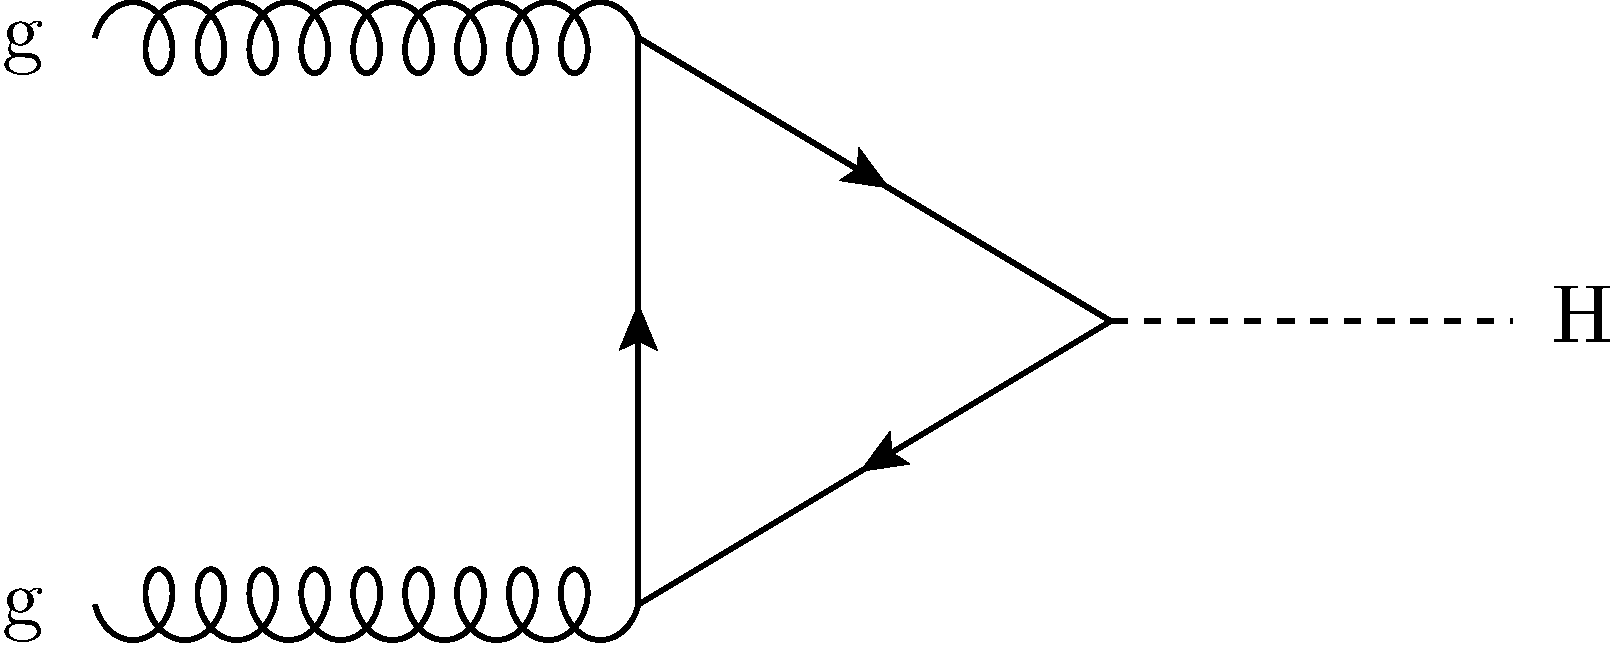
\includegraphics[width=0.45\textwidth]{Chapter01/Images/feynman_ggH.pdf}} \qquad
\subfloat[]{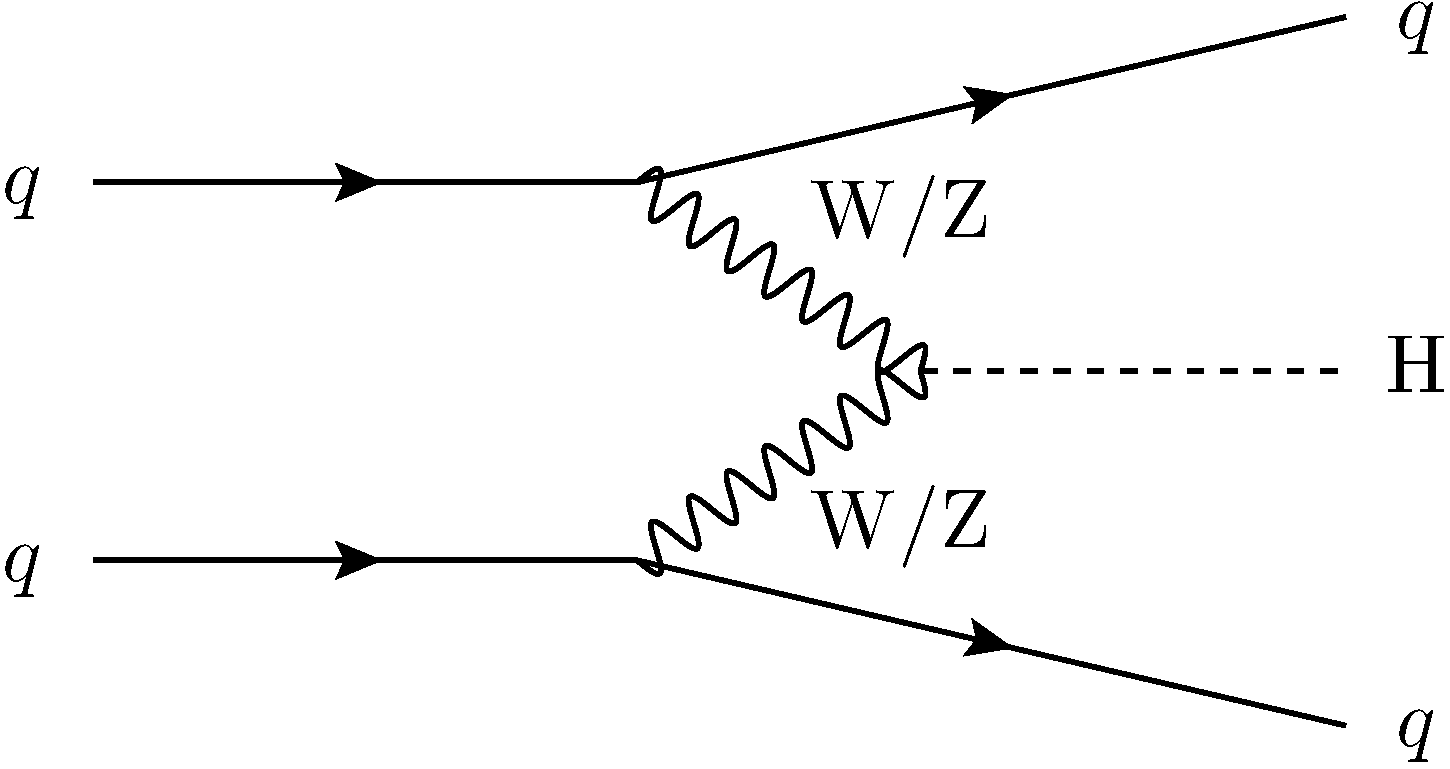
\includegraphics[width=0.45\textwidth]{Chapter01/Images/feynman_qqH.pdf}} \\
\subfloat[]{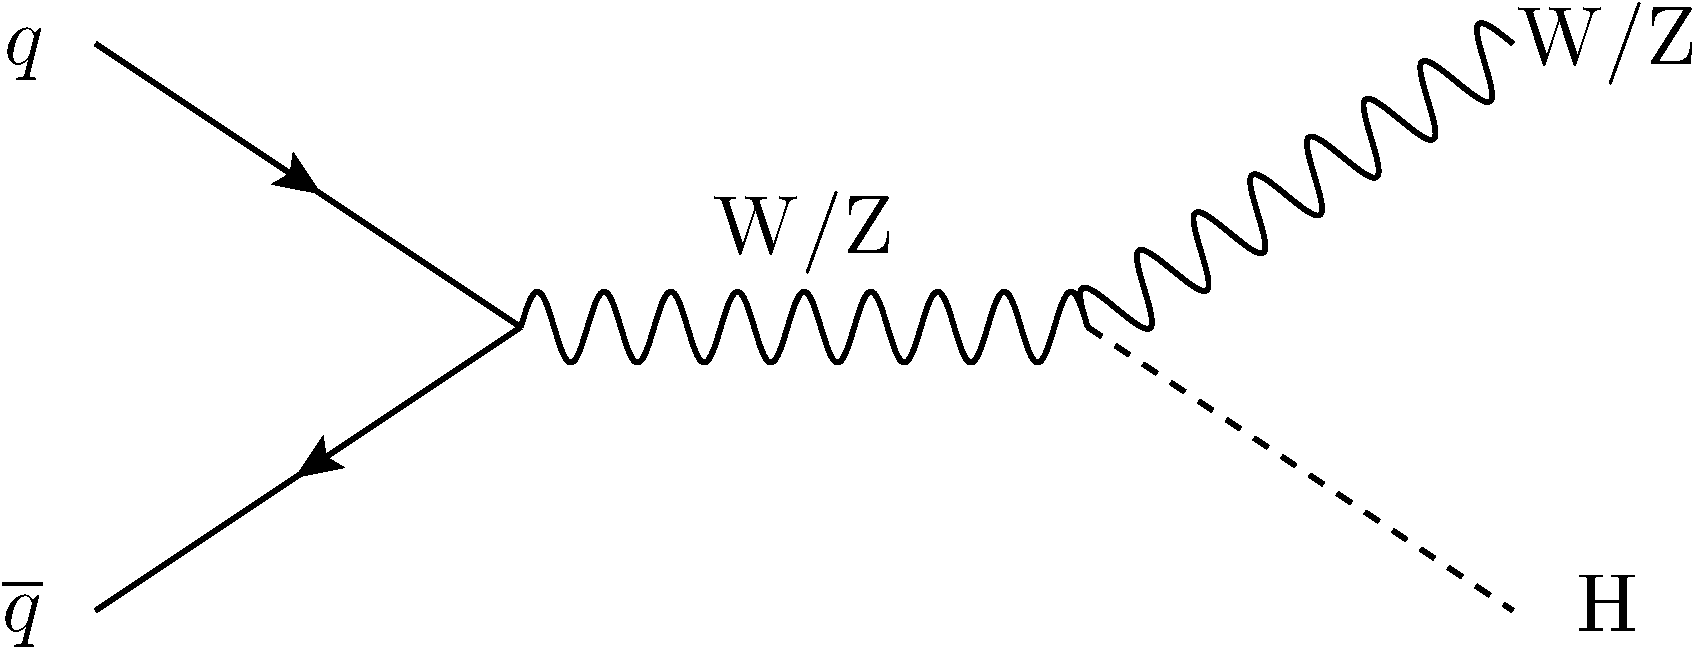
\includegraphics[width=0.45\textwidth]{Chapter01/Images/feynman_VH.pdf}}  \qquad
\subfloat[]{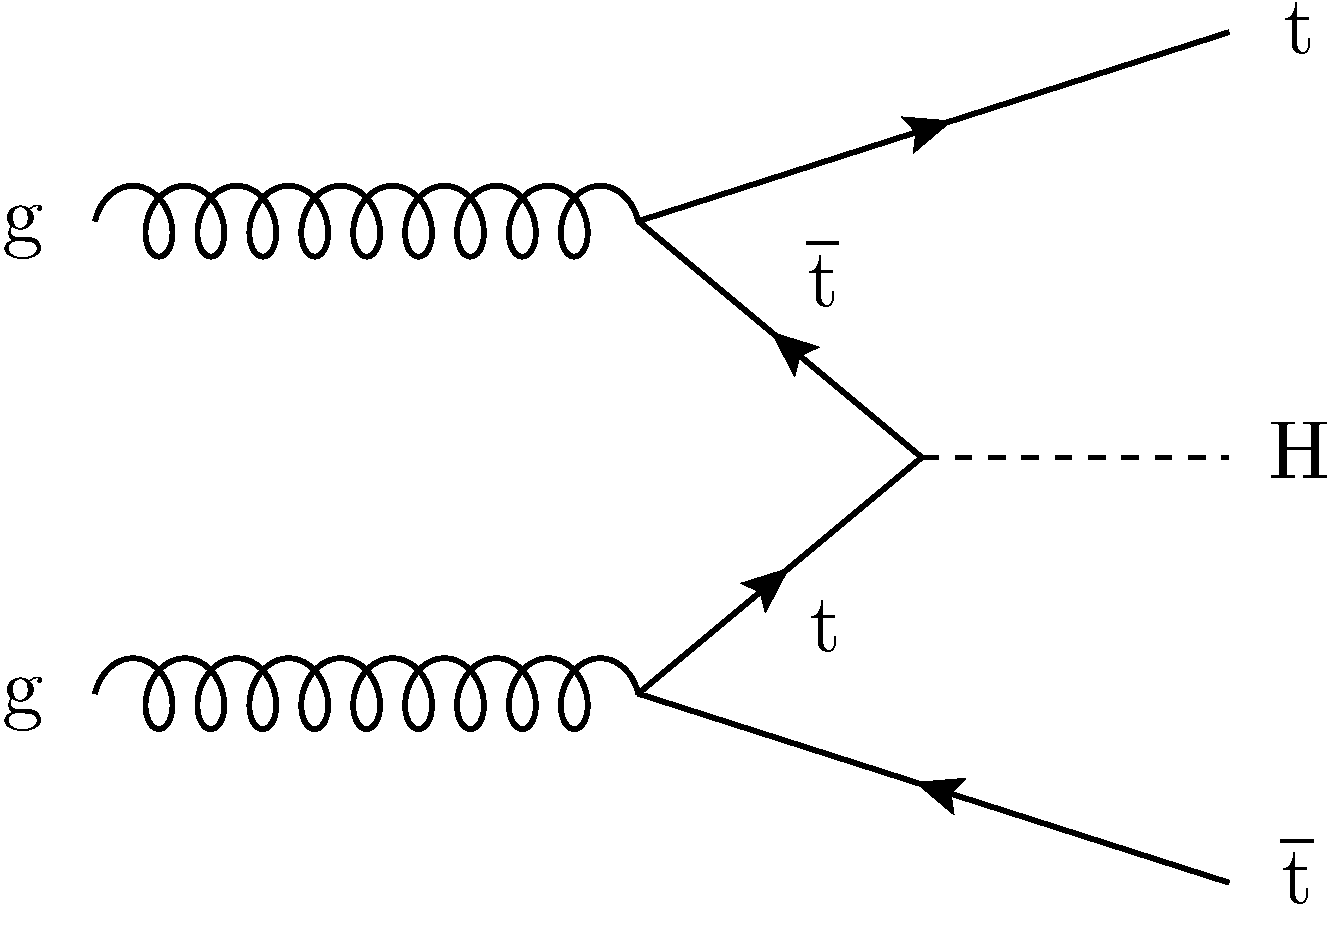
\includegraphics[width=0.45\textwidth]{Chapter01/Images/feynman_ttH.pdf}} \\
\caption[Feynman diagrams for the main production processes of the SM Higgs
boson.]{Feynman diagrams for the main production processes of the \gls{SM} Higgs
boson. Shown is (a) gluon fusion, (b) vector boson fusion and
associated production with (c) vector bosons and (d) top quarks.}
\label{FIGURE:Theory_SM_SearchingSMHiggs_SMFeynmanDiagrams}
\end{figure}

The production of the \gls{SM} Higgs boson in proton-proton collisions occurs primarily through gluon-gluon fusion, \gls{VBF} and associated production with either a vector boson or a pair of top quarks, the processes are illustrated in figure \ref{FIGURE:Theory_SM_SearchingSMHiggs_SMFeynmanDiagrams}. The Higgs boson only couple with particles that have mass, hence it does not couple to gluons which are massless. The gluon fusion production process goes mainly through a top quark loop. The top quark is the heaviest quark and thus also has the highest coupling with the higgs. All these four processes are accessible at the \gls{LHC}.

Searches for the Higgs boson have been already carried out at \gls{LEP} and the Tevatron. The \gls{LEP} was a particle accelerator colliding electrons and positrons at a center of mass energy ($\sqrt{s}$) between $90$ and $209\,\GeV$. For this type of colliding particles the dominant production channel is associated production with a $\PZ$ boson, this process is sometimes referred to as ``Higgsstrahlung''. In the experiments of the accelerator the searched performed were predominantly looking for decays to $\Pqb\Paqb$ and $\Pgtp\Pgtm$ pairs. The Higgs boson was not observed at \gls{LEP}, lead to the exclusion of a \gls{SM} Higgs with $m_{\PH}<114.4\,\GeV$ at the 95\% \gls{CL}~\cite{ARTICLE:LEPWorkingGroupforHiggsBosonSearches}.

Searches were also performed by the CDF and D0 Collaborations at the Tevatron accelerator, which collided protons and antiprotons with $\sqrt{s}=1.96\,\TeV$. The experiments performed searches in the mass range of $90-200\,\GeV$ over the Higgs boson decays $\Pqb\Paqb$, $\PWp\PWm$, $\gamma\gamma$ and $\Pgtp\Pgtm$ pairs, with the most sensitive being $\Pqb\Paqb$ and $\PWp\PWm$. The combined results of the Tevatron experiments resulted in an exclusion of a \gls{SM} Higgs boson with $m_{\PH}$ in the ranges $90-109\,\GeV$ and $149-182\,\GeV$~\cite{ARTICLE:CDFDOHiggsBosonStudies}. The results from the \gls{LEP} and Tevatron direct searches can be combined with precision measurements of electroweak observables at \gls{LEP} and by the \gls{SLD} to constrain the Higgs mass to $94^{+29}_{-24}\,\GeV$ \cite{SITE:lepewwg}, the quoted uncertainty only accounts for the experimental effects. Although, this value has been experimental excluded, the mass point where the Higgs boson would eventually be found is just about the upper one sigma error limit.

The \gls{LHC} is capable of colliding particles with a significantly higher centre of mass energy then the Tevatron. As a consequence it gives access to processes with smaller cross sections and allows searches in a wider mass range. Figure \ref{FIGURE:Theory_SM_SearchingSMHiggs_SMHiggsXS} shows the production cross section of different processes for proton-proton collisions with $\sqrt{s}=8\,\TeV$ as operated during the 2012 period of \gls{LHC} running. The dominant production process is  gluon fusion by over one order of magnitude in cross section, for most of the mass range. Other processes, even with such low relative production rate are also useful. Their topological characteristics can be exploited to isolate signal like event from the large quantities of background events. The second most likely process is the \gls{VBF} which is characterised by the presence of well separated high momentum quark jets. The associated production processes consist of a vector boson or a pair of top quarks in the final state, since these particles can decay to leptons and b-quarks, those modes allows for good background rejection. 

\begin{figure}[!htb]
 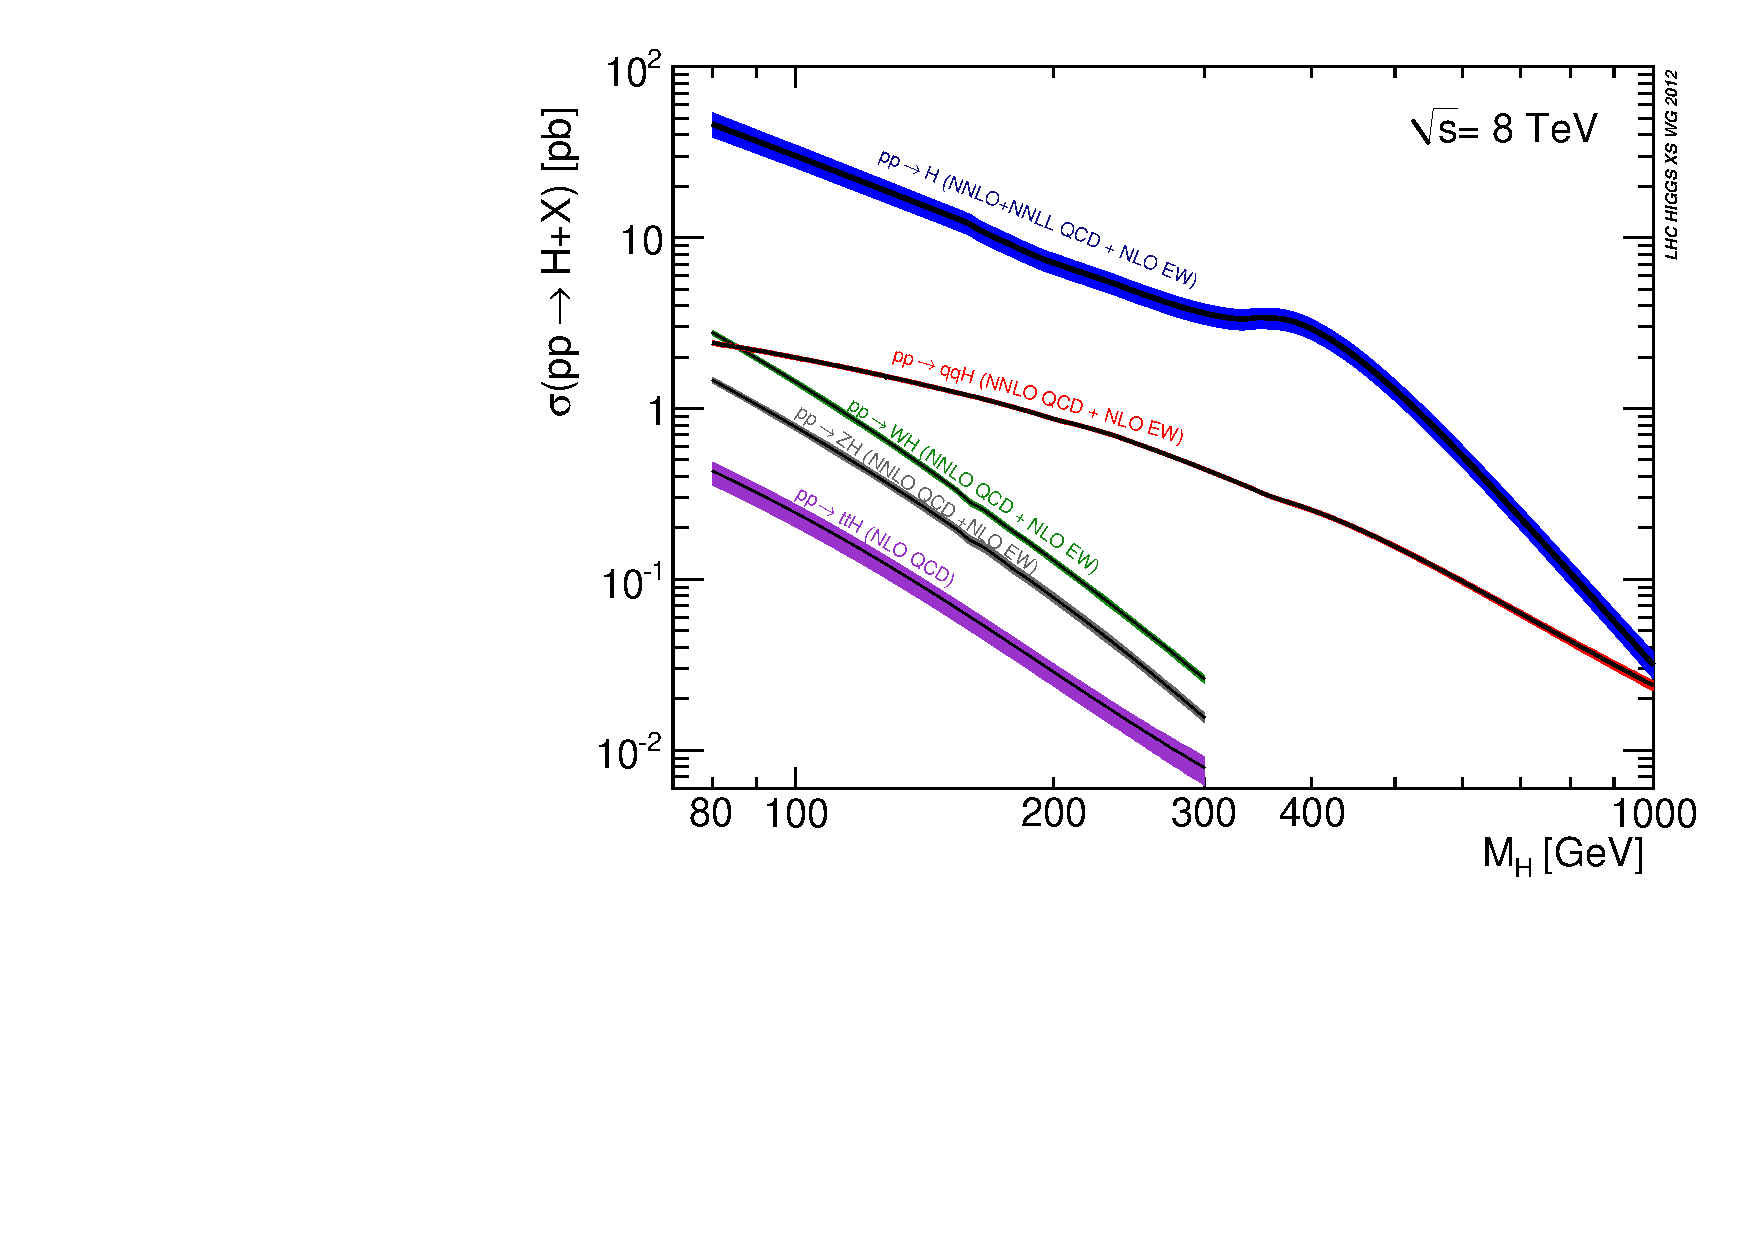
\includegraphics[width=0.7\textwidth]{Chapter01/Images/Higgs_XS_8TeV_lx.pdf}
\caption[Cross sections for Higgs production processes at $\sqrt{s}=8\,\TeV$ for
a range of Higgs boson masses.]{Cross sections for Higgs production processes at
$\sqrt{s}=8\,\TeV$ for a range of Higgs boson masses $m_{\PH}$~\cite{ARTICLE:HandbookofLHCHiggsCrossSectionsHiggsProperties}. Across the
mass range the gluon-fusion mode dominates, followed by the vector boson fusion
and associated production modes. The widths of the lines represent the
theoretical uncertainties on the cross section calculation.}
\label{FIGURE:Theory_SM_SearchingSMHiggs_SMHiggsXS}
\end{figure}

Figure \ref{FIGURE:Theory_SM_SearchingSMHiggs_SMHiggsBRs} shows the branching fractions to the different decay channels depending on the Higgs boson mass. At low Higgs boson mass, many possible decay channels are accessible. The decay into two photon, which cannot happen directly as the photon is massless, happens via a fermion or $\PW$ loops. Other decays are also possible to $\PWp\PWm$, $\PZ\PZ$, $\Pqb\Paqb$ and $\Pgtp\Pgtm$. For Higgs masses above $130\,\GeV$, decays to $\PWp\PWm$, $\PZ\PZ$ dominate as they becomes kinematically favourable. The observation of a Higgs boson in any of these decay channel is in itself important and gives a handle to probe the couplings of the particles involved in the Higgs production and decay. The most sensitive decay at the low mass region are $\Pphoton\Pphoton$ and $\PZ\PZ$ due to their clean signatures.

\begin{figure}[!htb]
 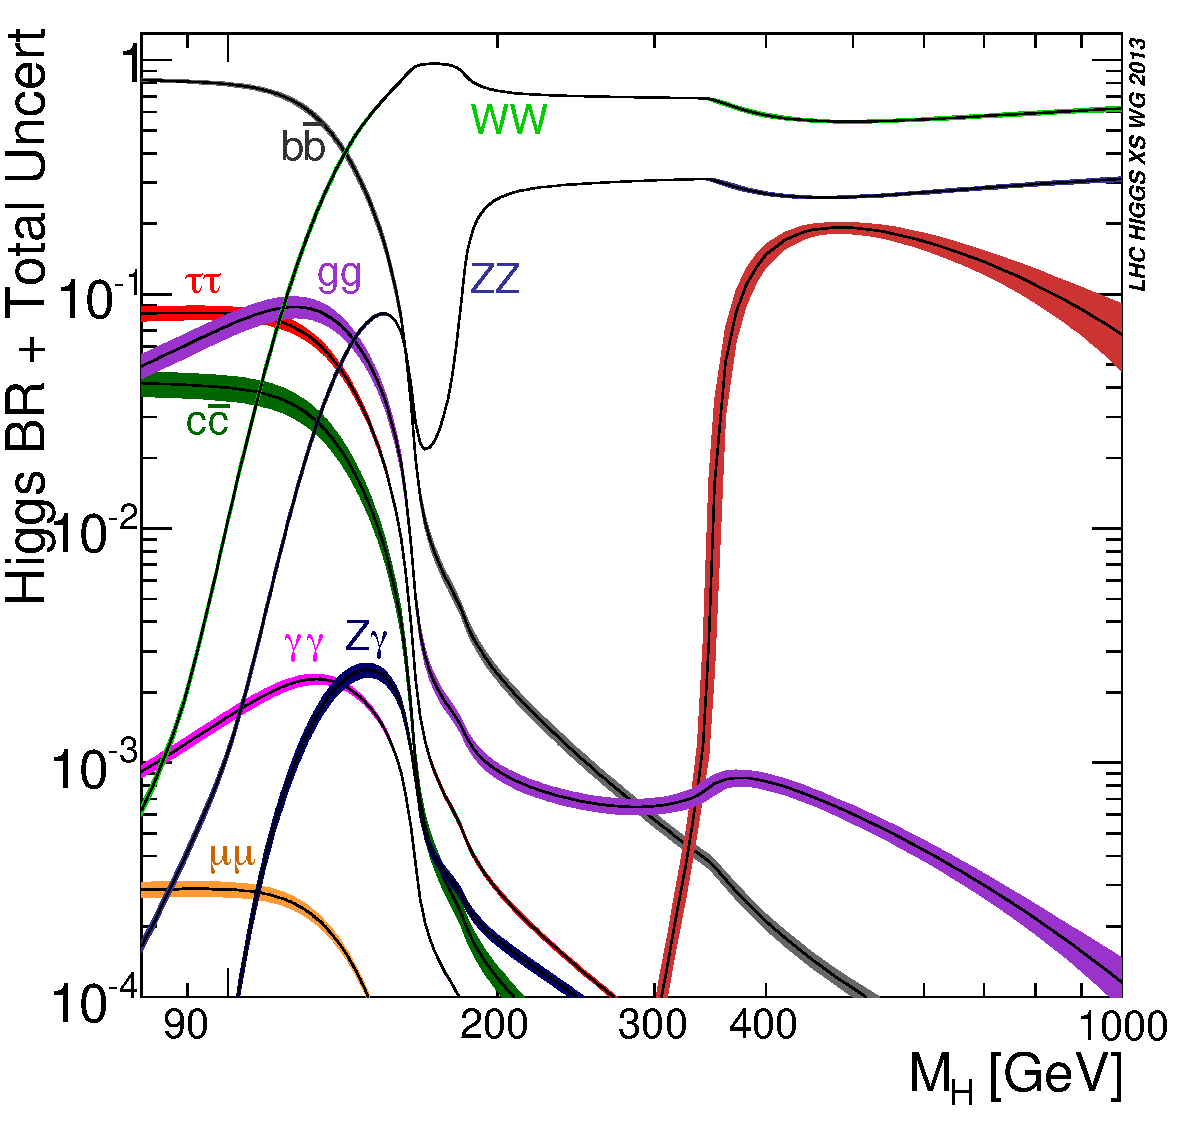
\includegraphics[width=0.6\textwidth]{Chapter01/Images/Higgs_BR.pdf}
\caption[Higgs boson branching ratios in the SM for a range of Higgs boson
masses.]{Higgs boson branching ratios in the SM for a range of Higgs boson
masses $m_{\PH}$ \cite{ARTICLE:HandbookofLHCHiggsCrossSectionsHiggsProperties}. At high masses, above their
kinematic thresholds, the $\PW\PW$,
$\PZ\PZ$ and $\ttbar$ (shown in red) decay modes dominate. 
At lower masses a wide range of different final states is possible. 
The widths of the lines represent the
theoretical uncertainties on the branching ratio calculation.}
\label{FIGURE:Theory_SM_SearchingSMHiggs_SMHiggsBRs}
\end{figure}

The ATLAS and CMS Collaborations announced the discovery of a new boson with a mass around $125\,\GeV$~\cite{ARTICLE:CMS_HiggsDiscovery,ARTICLE:ATLAS_HiggsDiscovery}. To achieve this result both experiments analysed approximately $5\,\invfb$ of data collected at $\sqrt{s}=7\,\TeV$ and $5-6\,\invfb$ at $\sqrt{s}=8\,\TeV$. This discovery was made by combining searches using $\PZ\PZ$ and $\Pphoton\Pphoton$ decay modes in both experiments, the observed combined excess of events yielded a $5\sigma$ deviation from the background-only expectation.

The \gls{LHC} Run I was completed in early 2013, with ATLAS and \gls{CMS} recording $\approx20\,\invfb$ at $8\,\TeV$. This increase in luminosity allowed access to less sensitive decay modes. The combination of both experiments $\PZ\PZ$ and $\Pphoton\Pphoton$ measurements results in best fit mass of $125.09 \pm 0.21(\text{stat}) \pm 0.11(\text{syst})\,\GeV$ and a signal strength relative to the \gls{SM} of $1.24^{+0.18}_{-0.16}$ \cite{ARTICLE:CombinedMeasurementOfTheHiggsBoson}. The \gls{CMS} collaboration has also performed a signal strength measurement combining the information from $\Pphoton\Pphoton$, $\PWp\PWm$, $\PZ\PZ$, $\Pqb\Paqb$, $\Pgtp\Pgtm$ and $\APmuon\Pmuon$ final states, obtaining a signal strength of $1.00\pm0.09(\text{stat})^{+0.08}_{-0.07}(\text{theo})\pm0.01(\text{syst})$~\cite{ARTICLE:CMScomb}. Individual channels were were studied in their compatibility with the \gls{SM}, and all of them show consistency is the \gls{SM} predictions for a $125\,\GeV$ Higgs boson. The ATLAS collaboration has also performed similar studies over production rates and couplings for various channels~\cite{Aad:2014eva,Aad:2014lwa,Aad:2015vsa}, and both collaborations have performed studies on the spin-parity quantum numbers~\cite{Chatrchyan:2013mxa,Chatrchyan:2013iaa,Aad:2013xqa} and limits have also been set over the invisible branching fraction which will be analysed in depth in this document. No significant deviations from the predictions of the \gls{SM} have been observed to date.

%%%%%%%%%%%%%%%%%%%%%%%%%%%%%%%%%%%%%%%%%%%%%%%%%%%%%%%%%%%%%%%%%%%%%%%%%%%%%%%%%%%%%%%
%%% SUBSECTION
%%%%%%%%%%%%%%%%%%%%%%%%%%%%%%%%%%%%%%%%%%%%%%%%%%%%%%%%%%%%%%%%%%%%%%%%%%%%%%%%%%%%%%%
\subsection{Invisible Higgs decay}
\label{SUBSECTION:Theory_SM_InvisibleHiggsDecay}

% STATUS: DONE (reviewed D. Colling x1)

The discovery of the Higgs boson described in the previous chapter, and the absence of any new experimental hints of new physics beyond the \gls{SM} at the \gls{LHC}, have strongly limited proposed models for new physics. Currently the uncertainties associated with the Higgs boson are still large enough to allow for the possibility of non-\gls{SM} properties. Although additional \gls{SM}-like Higgs bosons have been excluded over a wide range of masses, there is still the possibility of additional Higgs bosons with exotic decay modes.

Invisible Higgs boson decays are predicted in a wide range of models, for example in supersymmetric models to neutralinos \cite{ARTICLE:MSSMInvisibleHiggs} or graviscalars in models with extra dimensions \cite{ARTICLE:Graviscalars,ARTICLE:ADDInvisible}. If the Higgs boson can interact with the currently unknown dark matter sector, invisible decay modes could be possible, and bounds on these decays can constrain dark matter models.

The \gls{SM} Higgs boson can decay to neutrinos through $\PZ\PZ$ intermediate decay, but this decay has a very small branch ration of only 0.106\%. The observation of a significant branching fraction to invisible would be clear evidence of new physics and would point to direct production of dark matter.


